\begin{document}

\section{Introduction}
This project has set out to create an AI that is able to play Texas Hold'em Poker. The goal of the AI is to make as much money as possible while playing. For this project we built a Texas Hold'em Poker game in Python and trained several AI's to play the game. We rewarded them based on how much money they earned. The more the better!

Texas Hold'em Poker can be played by 2 to 9 player each with a bank of starting money. The initial setup before any play occurs is as follows: First a "dealer" button is placed in front of a player (can be one of the players physically next to the dealer), a "big blind" button is placed in front of the player to the left of the "dealer" button player, then to the "big blind" players left is the "small blind" player which receives a "small blind" button. These buttons are just tokens showing the previously mentioned words on them. They rotate clockwise after each hand is completed. Once these buttons are placed the big blind and small blind players pay their blinds and place the chips in front of them. Blinds are a set amount of money of x and 2x value. For example small blind of \$5 and a big blind of \$10. Next the dealer deals each player two cards, one at a time starting with the player with the "big blind" button in front of them. 

Once the cards are dealt the first main round begins. This round consists of players initial decisions. Each player has 5 main choices when making a decision. One they can fold their hand and get rid of their cards. They are no longer in the hand. Two they can check if there is no bet they are required to match. Three they can bet an amount of money that is larger than the minimum bet and smaller or equal to what they have in their bank, if no other player has bet before them. Four, if another player has bet before them they can call the bet and match the bet with money from their bank. Five, they can raise the bet and add more money to the previous players bet. Once all the players have made their decisions and all decisions have been resolved and we reach the last player than needs to act the round is over. 

Starting the second round is the dealer who burns a card then deals three of the five community cards. This is referred to as the "flop". Once the three cards are shown another round of decisions are made by the players. Once all the decisions are resolved the round is over.

Starting the third round is the dealer who burns a card then deals one more community card. This is referred to as the "turn". Once the new community card is shown another round of decisions is made by the players. Once all the decisions are resolved the round is over.

Starting the fourth and final round is the dealer who burns a card then deals one more community card. This is referred to as the "river". Once the new community card is shown a final round of decisions is made by the players. Once all the decisions are resolved a winner is determined. The winner is determined by the player with the best 5 card hand. The hand order is shown in INSERT HAND VALUE FIGURE. If two players have the same level of hand the one with the highest card value wins. For example if two players have straights, one player has 3,4,5,6,7 and the second player has 4,5,6,7,8 the second player would win.

Some notes, play can end sooner than the fourth round if all but one player folds. If a player wants to call or raise using all their chips its called going "all in". If a player who is all in loses and has no more money in their bank they are out of the game.

The AI in this case will have all the information about the current state of the game and make one of the previously discussed decisions. After a number of hands the AI will be judged and then the best performers are chosen for the next generation. This process will repeat until a set stopping criteria.


\section{Related Work}
Ever since computers have been around have we been pitting them against humans in all manners of games. Some famous examples are chess AI and GO AI that have defeated the worlds best humans at these games\cite{brown2017libratus}\cite{gilpin2005optimal}\cite{doi:10.1126/science.aay2400}. Poker is just another game waiting to be conquered by computers. However it presents a different type of game compared to chess and GO. The later games are perfect information games meaning that both (all) players can see the complete state of the game/board. Poker however is an imperfect information game meaning that one player can not have/see the complete state of the game/board\cite{brown2017libratus}\cite{davidson2000improved}\cite{gilpin2005optimal}\cite{gilpin2006competitive}\cite{doi:10.1126/science.aay2400}. This forces the AI to have to guess about what action to take since they do not have all the information. This has been the trickiest part of making an unbeatable poker AI. This task also applies to many real world applications that also deal with imperfect information.

In order to solve this problem many different approaches have been taken. "Libratus: The Superhuman AI for No-Limit Poker" has taken a three module approach to the problem\cite{brown2017libratus}. Libratus consists of a pre-computing module, a nested sub-game solver module and a self improvement module. The first module deals with the general strategy of the AI and makes categories of all the possible situations and actions that could be made from that point. It has two kinds of abstractions that it groups these situations into: action abstraction and card abstractions\cite{brown2017libratus}. The card abstractions deal with the possible card combos at each stage of play and lumps groups of card possibilities into buckets that millions of card combos. This is only employed on the last two rounds of play\cite{brown2017libratus}. The use of abstractions gives the AI a general game plan and one that will be refined in the second module. The abstracted game that is created in this module is solved with a distributed version of an improvement over Monte Carlo Counterfactual Regret Min-imization (MCCFR)\cite{brown2017libratus}.

The second module examines the game at a finer detailed level to make the best decision it can. Since an imperfect information game cannot be solved on its own the AI second module looks at sub games similar to the one that it is trying to solve and uses that information to make its decision\cite{brown2017libratus}. The third and final module is the self improvement model. It uses the previous data and the outcome of the most recent hand to fine tune its performance. It learns what sub games it should have used and how to arrive at that conclusion in the future\cite{brown2017libratus}.

Another approach is taken by "Poki" which is a poker AI that specifically focuses on opponent modeling\cite{davidson2000improved}. Poki's goal is to keep track of how opponents are playing, how it expects them to play and to react to these factors. Poki uses an artificial neural net to keep track of and predict its opponents actions. Poki used feed-forward and back propagation algorithms to tune the model. This model had much better results at predicting opponents actions than previous attempts\cite{davidson2000improved}.

Another approach uses "Rhode Island Hold’em Poker" to accomplish the goal of training a poker playing AI. Rhode Island Hold'em Poker is a simplified version of Texas Hold'em Poker than contains less possible states the game can be in making the imperfect information problem easier to solve\cite{gilpin2005optimal}. The goal for this approach is to train and develop models on a less complex version of the imperfect information problem so that these models can become really good at this version quicker and more efficently before being applied to the more complex problem\cite{gilpin2005optimal}.

From looking into all these different approaches we decided to combine a few and apply a neural net to a slightly simplified version of Texas Hold'em Poker. Where our focus was on the decision making of the AI to make the most money possible.

\section{Approach}
\subsection{Data/Problem Analysis}
The data in this problem is poker hands, games and the results of them. We did not use any historical data for this solution. All data was used for the AI learning while it played the game. We valued AI that could win the most money. NATHAN MAYBE SOMETHING HERE ABOUT THE VALUE FUNCTION??? IT COULD GO LATER

\subsection{Resources Used}
Our programming language of choice is the same as the one from this class, Python 3. We used several libraries and they can be found in the below table \autoref{tab:libs}. The most important of these is the Neat library. The Neat library is the one that we use for the AI. NATHAN ALSO FINISH THIS PLEASE
\begin{table}[H]
    \caption{Python Libraries Used}
    \centering
    \begin{tabular}{ | l |}
    \hline
        Library name \\
        \hline
        \hline
        numpy \\
        itertools \\
        tensorflow.keras \\
        neat \\
        logging \\
        pytest \\
        functools \\
        graphvis \\
        warnings \\
        matplotlib.pyplot \\
        os \\
        copy \\
        
    \hline
    \end{tabular}
    \label{tab:libs}
\end{table}

\subsection{Software Design}
Our software design was a bottom up object oriented design. There is two halves to solution. One half is the poker game itself and the second half is the AI that can play the poker game. The first half, the poker game was built bottom up objected oriented starting with the basic building blocks of the poker game. First a card was implemented then a deck. From there the logic of the game was implemented in pieces where each piece added more complexity. Pieces include, players, hands, community cards, board, hand values, rounds and games etc. 

Once the game was complete the next step was adding the Neat integration to create the AI player. NATHAN FINISH THIS PLEASE

\clearpage
% THIS WILL HAVER TO BE PLAYED WITH
\begin{figure}[H]
    \centering
    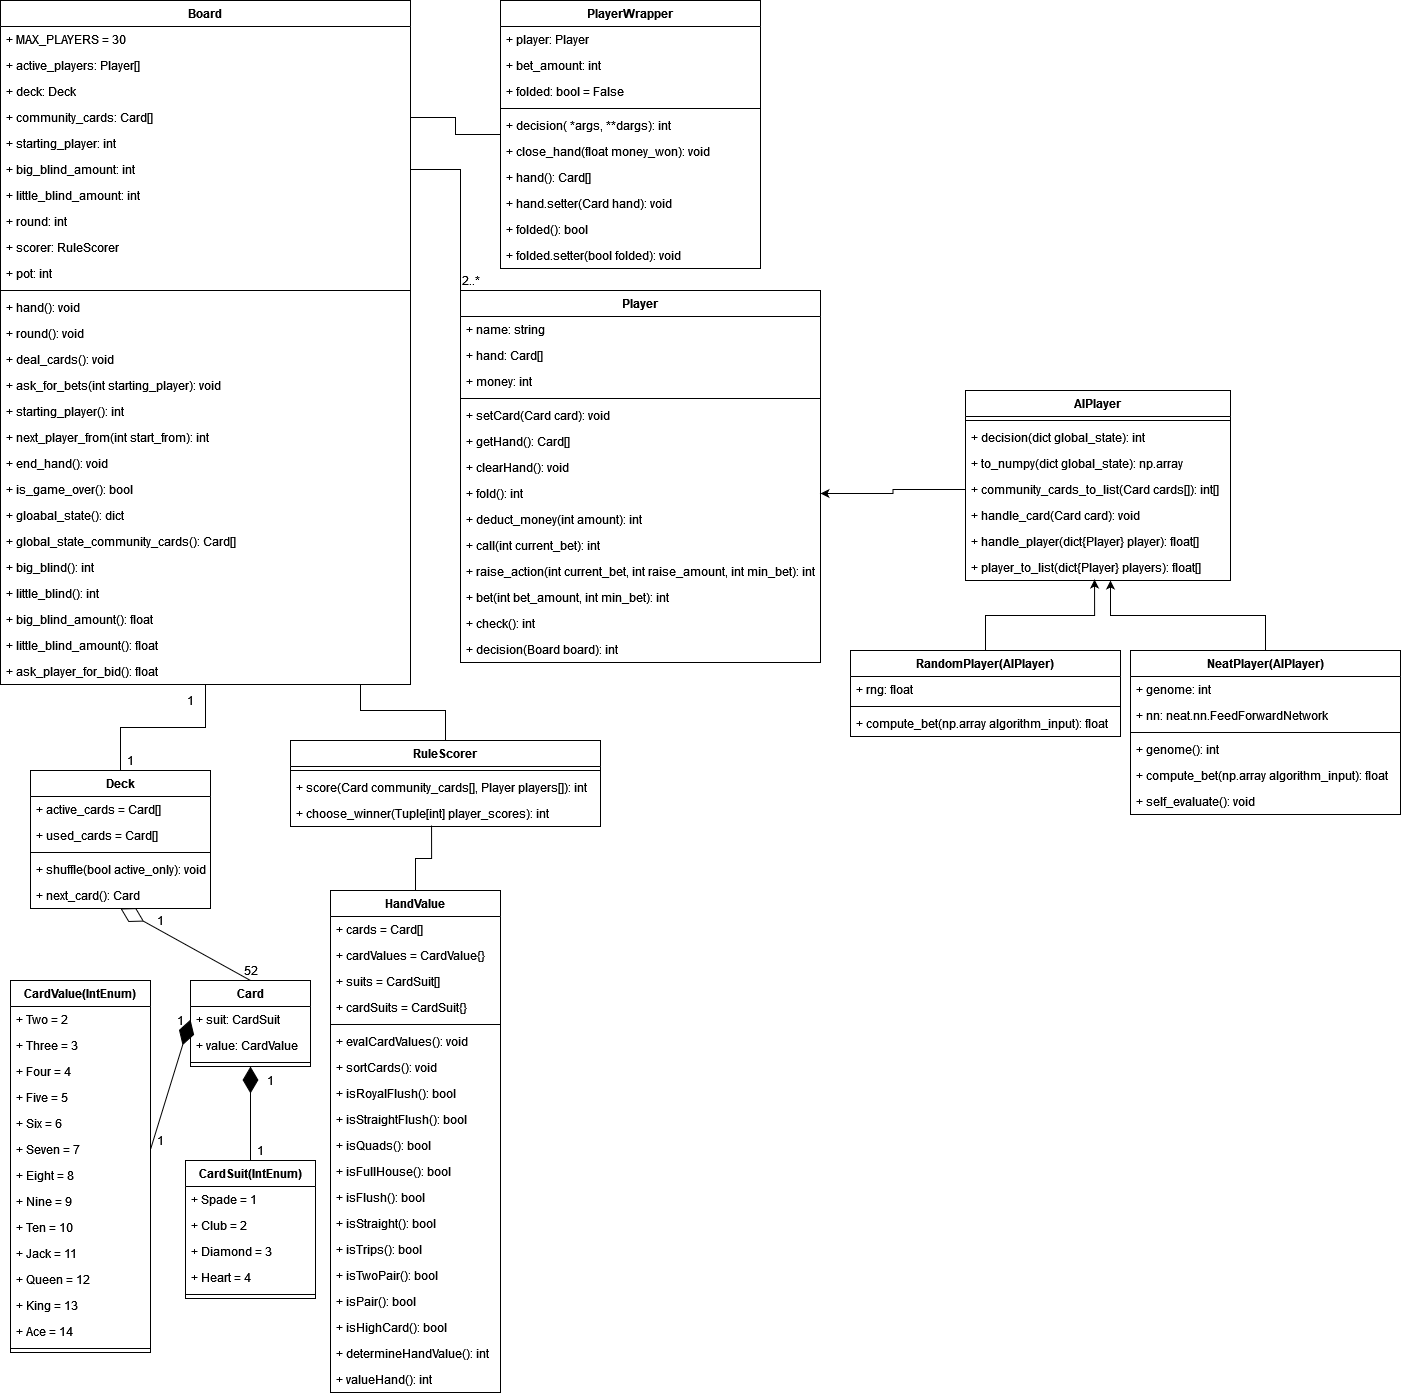
\includegraphics[scale=0.4]{resources/Poker_AI_-Class_Diagram.drawio.png}
    \caption{Class Diagram for our Poker AI}
    \label{fig:classDiagram}
\end{figure}
% \image{resources/Poker_AI_-Class_Diagram.drawio.png}{Class Diagram for our poker AI}{fig:classDiagram}



\subsection{Source Code Description}
\begin{table}[H]
    \caption{Source Code Files}
    \centering
    \begin{tabular}{ | c | p{14cm} |}
    \hline
         File Name & Description \\
        \hline
        \hline
        main.py & The driver of the program\\ \hline
        visualize.py & Creates the graphs and visuals\\ \hline
        AIPlayer.py & Implements AI Player class both random and Neat player\\ \hline
        Board.py & Poker board (table) implementation. All the control logic for how the game is played is handled here\\ \hline
        Card.py & A playing card implementation\\ \hline
        Deck.py & Deck of Cards implementation\\ \hline
        HandValue.py & Evaluator for hands value. Uses the official poker ranking for determining hand value\\ \hline
        Player.py & Poker Player functionality. Fold, check, bet, raise, call, cards in hand and money\\
        Mock\_player.py & \\ \hline
        test\_AIPlayer.py & Test cases for the AIPlayer Class \\ \hline
        test\_Board.py & Test cases for the Board Class\\ \hline
        test\_Card.py & Test cases for the Card Class\\ \hline
        test\_Deck.py & Test cases for the Deck Class\\ \hline
        test\_HandValue.py & Test cases for the HandValue Class\\
        
    \hline
    \end{tabular}
    \label{tab:sourceCode}
\end{table}

\section{Evaluation and Results}

\subsection{Results}

\subsection{Results Discussion}

\section{Conclusion}


\section{References}
\printbibliography

\section{Appendix: Personal Contribution and Lessons Learned}
\subsection{JP}
My personal contributions were to the brainstorming and deciding on the topic for the project, helping design the implementation of Texas Hold'em Poker in Python 3, creating and formatting the presentation, creating and the initial formatting of the final report. Writing the introduction, related works, a portion of the approach section, created the class diagram, creating the file description table, compiling the libraries used table. For the implementation I specifically wrote the hand value and player classes for the Texas Hold'em Poker Game as well as the tests for these class.

For lessons learned. I learned that the power and capabilities of a poker playing AI is really interesting and hard to get a complete one working. I discovered this while reading all the previous research and seeing how far they have come but also how far they have to go. The idea of an imperfection information problem is nothing new to humans and I believe we are uniquely suited for that kind of problem but computers are not. They are designed for complete information problems. When dealing with incomplete information problems with computers is where the human inspired neural networks come into play and they have had the most success in these problems. Early computers were just not powerful enough. So knowing where they came from to see Nathan and I be able to create pretty decent Texas Hold'em AI players is pretty neat (pun intended). Although we used a slightly simplified version it is still really rewarding to see the outcome. 

One thing I did not expect was that during our training and testing of the models there was original one AI just completely destroyed the random AI. I would have expected it to take a while to learn a decently complex game. From this we put several AI players against each other instead of having the random AI and it improved all the AI players. It was really interesting to see the growth of the best AI model over generations of its development. Some times it was really clear who the best was and sometimes it was back and forth or sometimes the AI would regress in skill, which I did not think it would do.
\subsection{Nathan}


\end{document}